\subsection{Información general del MCU}


En la siguiente práctica de laboratorio se utiliza el microcontrolador de ATmel ATmega328P como
elemento central de la práctica. El mismo posee las siguientes características \cite{ppt}:

\begin{itemize}
    \item Microcontrolador AVR de 8 bits.
    \item Arquitectura RISC/Harvard.
    \item 4/8/16/64Kb Flash, 512b/1/2k bytes de
SRAM y 256/512/1k bytes de EEPROM.
\item 23 GPIOs.
\item Timer/Counters de 8 y 16 bits e interrupciones.
\item 8 canales PWM y comparador
analogico y 6 canales 10-bit ADC.
    
\end{itemize}






\begin{figure}[H]
\centering
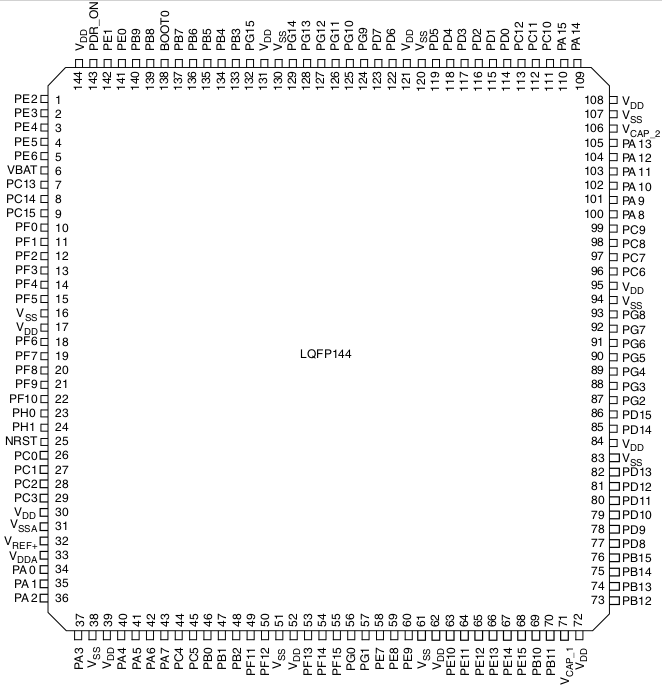
\includegraphics[scale=0.8]{./images/pines.png} 
\caption{Diagrama de pines ATmega328P \cite{mcu}.}
\label{f1}
\end{figure}

\begin{figure}[H]
\centering
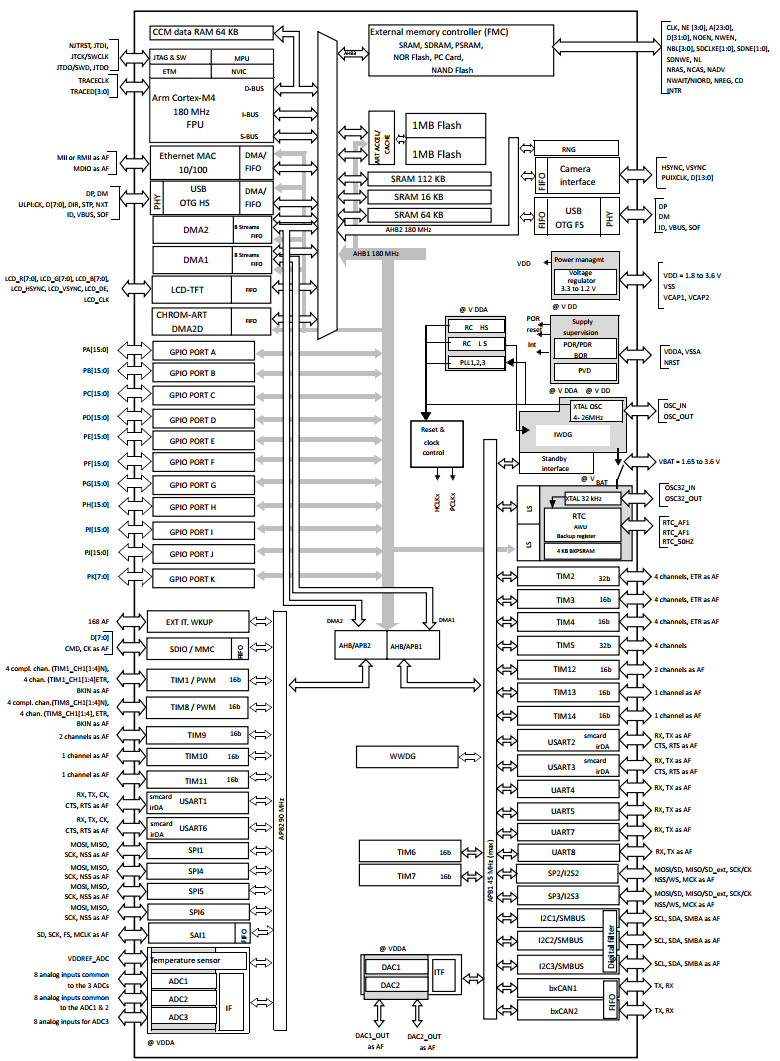
\includegraphics[scale=0.75]{./images/bloques.png} 
\caption{Diagrama de bloques ATmega328P \cite{mcu}.  }
\label{f1}
\end{figure}


\subsubsection{Sobre la placa Arduino UNO Rev3}
Arduino UNO es una excelente opción para iniciarse en la electrónica y la codificación, siendo la más utilizada de la familia de Arduinos.\\
Consta de 14 pines de entrada/salida digital (de los cuales 6 se pueden usar como salidas PWM), 6 entradas analógicas, un resonador cerámico de 16 MHz (CSTCE16M0V53-R0), una conexión USB, un conector de alimentación, un cabezal ICSP y un botón de reinicio. \cite{arduino}\\
Adicionalmente Arduino proporciona la siguiente información
% Please add the following required packages to your document preamble:
% \usepackage[table,xcdraw]{xcolor}
% If you use beamer only pass "xcolor=table" option, i.e. \documentclass[xcolor=table]{beamer}
% \usepackage[normalem]{ulem}
% \useunder{\uline}{\ul}{}
\begin{table}[H]
\centering
\begin{tabular}{|c|c|}
\hline
Microcontroller   & {ATmega328P}               \\ \hline
Operating Voltage           & 5V                                                    \\ \hline
Input Voltage (recommended) & 7-12V                                                 \\ \hline
Input Voltage (limit)       & 6-20V                                                 \\ \hline
Digital I/O Pins            & 14 (of which 6 provide PWM output)                    \\ \hline
PWM Digital I/O Pins        & 6                                                     \\ \hline
Analog Input Pins           & 6                                                     \\ \hline
DC Current per I/O Pin      & 20 mA                                                 \\ \hline
DC Current for 3.3V Pin     & 50 mA                                                 \\ \hline
Flash Memory                & 32 KB (ATmega328P) de los cuales 0.5 kB para bootloader \\ \hline
SRAM                        & 2 KB (ATmega328P)                                     \\ \hline
EEPROM                      & 1 KB (ATmega328P)                                     \\ \hline
Clock Speed                 & 16 MHz                                                \\ \hline
LED\_BUILTIN                & 13                                                    \\ \hline

\end{tabular}
\caption{Características eléctricas y generales de la tarjeta Arduino UNO \cite{arduino}.}
\label{t1}
\end{table}


\begin{figure}[H]
\centering
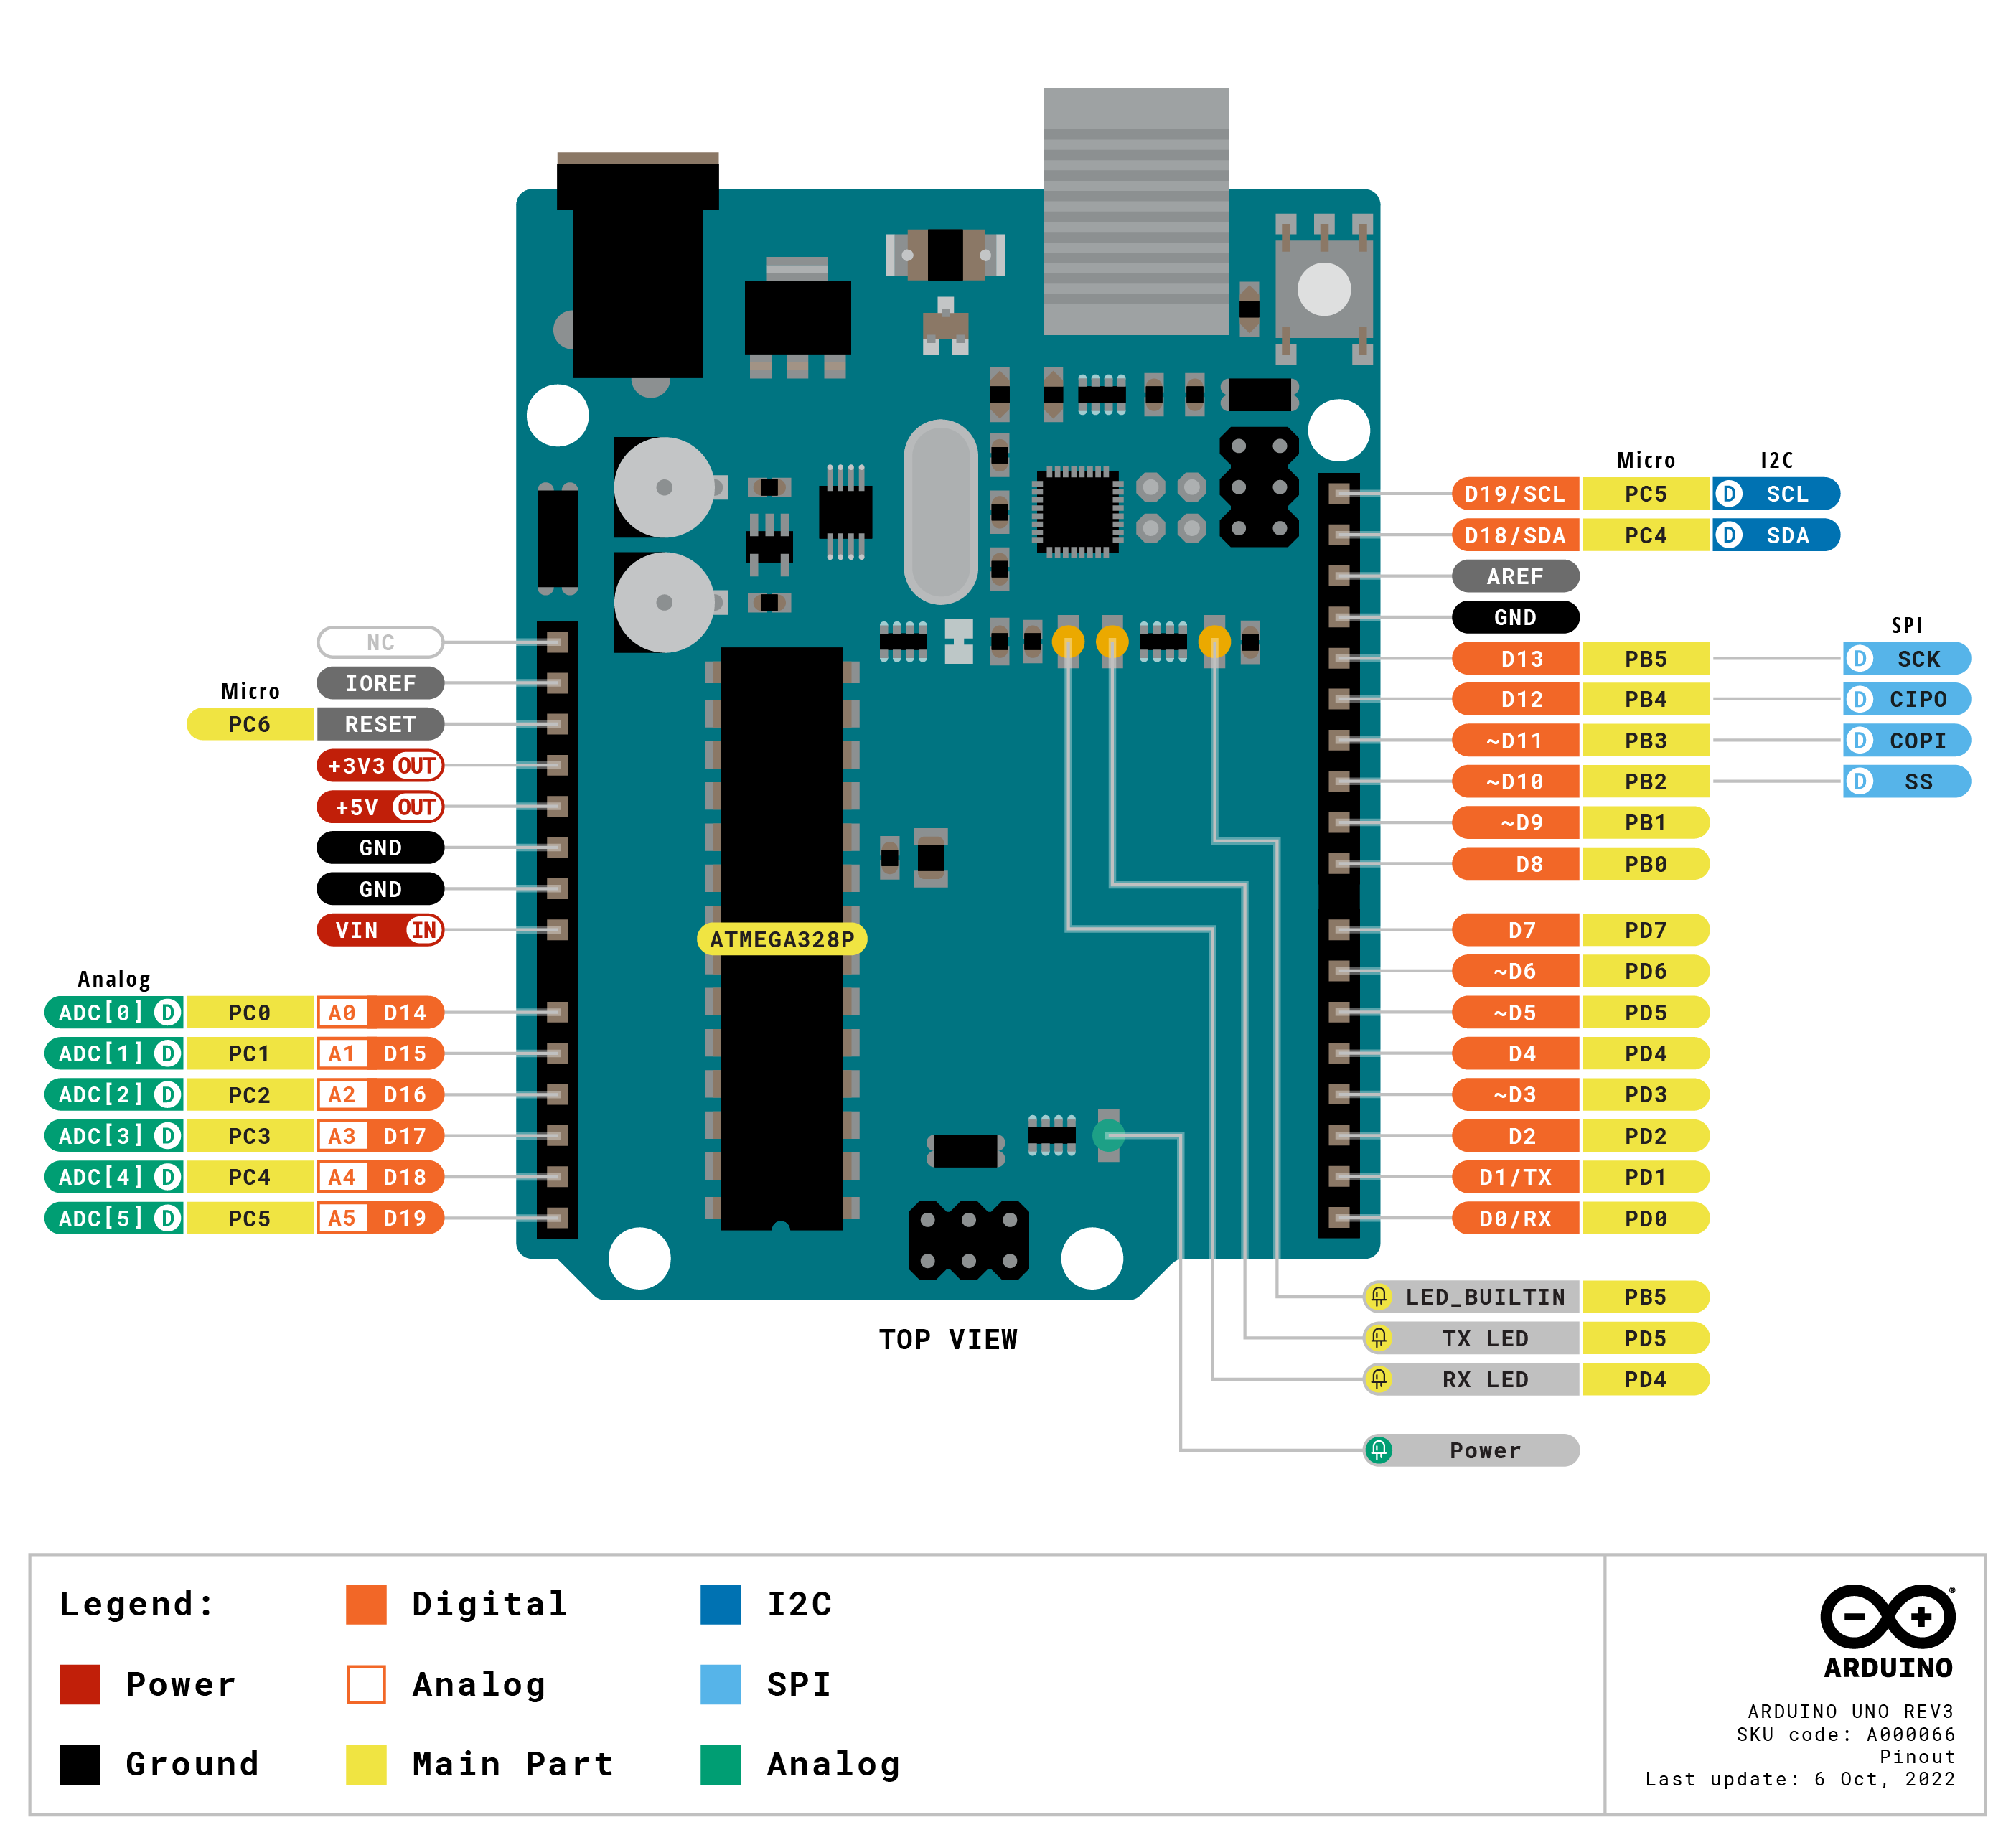
\includegraphics[scale=0.6]{./images/aaa.png} 
\caption{Diagrama pinout de Arduino UNO Rev3 \cite{arduino}.}
\label{f1}
\end{figure}